\chapter{Evaluation of NMR data for examining IL-10-GAG interaction}

The combination of both, \textit{in silico} methods and nuclear magnetic
resonance (NMR) data, often leads to an improved understanding of the system
under investigation, compared to the insights obtained with either approach
individually. This is especially true for protein-GAG systems, where \textit{in
silico} simulations are usually performed based on NMR data in order to obtain a
structural model with larger spatial resolution than achievable from NMR data
alone. The principal complementarity of NMR and \textit{in silico} methods with
respect to protein-GAG systems is broad and has been demonstrated and published
before, for instance in \cite{pichert_characterization_2012, sost_heparin_2009,
nieto_conf_selection_heparin_2011}.

In an ongoing effort, G. Künze from Prof. D. Huster's laboratory at the
Universität Leipzig investigates the IL-10-GAG system with NMR methods. In this
chapter, I describe how I post-processed his nuclear Overhauser effect
spectroscopy data in order to derive heparin tetrasaccharide structure models
for the free state (without IL-10 in solution) and bound state (with IL-10 in
solution) and discuss the implications of the corresponding results. This work
is part of our collaborative publication titled \enquote{NMR characterization of
the binding properties and conformation of glycosaminoglycans interacting with
interleukin-10} in the \textit{Glycobiology} journal \cite{kuenze_gehrcke_2014}.
Additionally, in this chapter I summarize further insights derived from G.
Künze's data and discuss them in the context of the conclusions drawn in this
thesis so far.

%The combination of insights gained via \textit{in silico} methods and
%experimentally obtained data has led to an improved understanding of the
%molecular recognition principles governing the IL-10-GAG system. This chapter
%presents the studies and outcomes of this collaborative effort.

\section{Heparin structure calculation for the bound and unbound state}

\subsection{Background: NOESY for inter-atomic distance determination}
\label{nmr:noesy_background}

In essence, the spins of atomic nuclei that are spatially close to each other
(closer than about \SI{5}{\angstrom}) may undergo a significant dipole-dipole
interaction, leading to the measurable effect of nuclear spin polarization
transfer from one nuclear spin population to another. In other words, after
excitation, two dipolar-coupled spins do not relax independently, which is
called the nuclear Overhauser effect (NOE). In two-dimensional nuclear
Overhauser effect spectroscopy (NOESY) experiments, this correlation effect
manifests itself in form of off-diagonal resonance peaks. In first order
approximation (or \enquote{isolated two-spin approximation}), the intensity of
such a so-called cross peak is proportional to the cross-relaxation rate
constant for the two-spin system. Due to the dipolar nature of this spin-spin
interaction, the rate constant is proportional to the inverse sixth power of
the distance between the two spins \cite{neuhaus2000_noe}. Likewise, the main
usage of the nuclear Overhauser effect in NMR spectroscopy for biological
questions is the detection of distances between pairs of protons. Eventually and
under ideal conditions, NOESY can be used for collecting sufficient geometrical
information about a certain molecule for determining a three-dimensional
structure of that molecule (obviously, this requires knowledge about the
chemical configuration of that molecule as well as a mapping between cross peaks
and atom pairs). In practice, depending on the environmental conditions and on
the type of molecule investigated, there are various sources of error that can
prevent NOE cross peaks from building up, or that significantly invalidate the
assumption of a linear dependence between the peak intensity and the relaxation
rate constant \cite{palmer_online_nmr_relaxation}, affecting at least the
spatial resolution of the data, or even the ability to obtain meaningful NOE
data at all.


\subsection{Methods} G. Künze carried out nuclear Overhauser effect spectroscopy
experiments for measuring GAG-internal hydrogen-hydrogen (${}^1$H-${}^1$H) NOE
cross peaks of heparin tetrasaccharide (HP dp4) molecules in solution, in two
different conditions: once under presence of \hl{(murine)} IL-10 in the very
same solution, and once without presence of IL-10. The protocol details of these
experiments have been published in \cite{kuenze_gehrcke_2014}. The aim of these
experiments was to extract and use the geometry information encoded in the
resulting NOESY data, for creating two HP dp4 structure models: one for what we
call the \enquote{bound} state, and one for the \enquote{unbound} state (with
and without IL-10, respectively).

The creation of structure models from the NOESY-derived distance data can be
considered an optimization problem --- with the goal of finding the heparin
structure fulfilling the experimentally obtained cartesian distance constraints
as good as possible. I have approached this optimization problem with simulated
annealing molecular dynamics simulations, which is a classical method applicable
in this scenario \cite{nilges_sim_annealing_noe_1988}.

HP dp4-internal ${}^1$H-${}^1$H distances were calculated from experimentally
obtained NOE intensities assuming a $1/r^6$ distance dependence between
interacting protons, as justified in \cref{nmr:noesy_background}. The
calibration was based on the H2-H4 and H3-H5 proton pairs of the GlcNS,6S ring
(atom nomenclature according to IUPAC rules) with a known distance of
\SI{2.55}{\angstrom} in the ${}^4$C${}_1$ chair conformation. A tolerance
interval of $\pm \SI{0.3}{\angstrom}$, $\pm \SI{0.6}{\angstrom}$ and $\pm
\SI{1.0}{\angstrom}$ was specified for measured distances $<
\SI{2.0}{\angstrom}$, between \num{2.0} and $\SI{4.0}{\angstrom}$, and $>
\SI{4.0}{\angstrom}$, respectively. The corresponding raw distance data is
enlisted in the supplementary material of \cite{kuenze_gehrcke_2014}.

The experimentally obtained distance restraints were subsequently used for GAG
structure determination using MD simulations employing the NMR restraint
functionality implemented in the PMEMD module of Amber 12 \cite{case_amber_12}.
Atom types of the GLYCAM 06g force field \cite{kirschner_glycam06:_2008} were
used to build the heparin tetrasaccharide IdoA,2S-GlcNS,6S-IdoA,2S-GlcNS,6S,
referred to as rings A, B, C, D, respectively. Sulfate partial charges, which
are not provided within GLYCAM, were obtained from RESP calculations for
methylsulfate at the 6-31(d)G level of theory --- in consistence with the other
parts of the force field. The heparin molecules used in the NMR experiments were
prepared by enzymatic digestion, so the non-reducing terminal uronic acid became
unsaturated. Since GLYCAM does not contain proper parameters for 4,5-unsaturated
uronic acid, we modeled the non-reducing terminal acid as IdoA,2S and NOE
signals involving hydrogens of ring A other than H1 were not applied as
restraints in the simulations. Generally, the structure generation was performed
in a two-step protocol, first by structure optimization in implicit solvent, and
subsequent refinement in explicit solvent. The two stages were repeated many
times, yielding an ensemble of structure models.

The first structure optimization stage was a simulated annealing protocol using
a simple implicit solvent model with a $1/r$ distance dependency of the
dielectric constant. The protocol contained the following steps: \textit{i)}
steepest descent and conjugate gradient minimization without restraints,
\textit{ii)} 100 ps MD with tight coupling to a \SI{600}{\kelvin} heat bath and
gradual activation of NMR distance restraints, \textit{iii)}
\SI{300}{\pico\second} MD with restraints, gradual temperature change from
\SI{600}{\kelvin} to \SI{10}{\kelvin}, and normal coupling to heat bath,
\textit{iv)} short MD with gradual cooling to \SI{0}{\kelvin} and tight coupling
to heat bath. The MD time step for this protocol was set to
\SI{1}{\femto\second}. The second optimization stage was performed with periodic
boundary conditions in TIP3P explicit solvent (with at least \SI{8}{\angstrom}
from all solute atoms to the box boundary), with Na+ ions for system
neutralization, using SHAKE, and with an MD time step of \SI{2}{\femto\second}.
The following steps were performed: \textit{i)} solvent minimization with
constrained solute, \textit{ii)} \SI{20}{\pico\second} heat up MD to
\SI{300}{\kelvin} in NVT ensemble with strong positional restraints on solute
atoms, \textit{iii)} \SI{200}{\pico\second} equilibration MD in NPT with weak
positional restraints on solute atoms and NMR distance restraints, \textit{iv)}
\SI{200}{\pico\second} MD in NPT with NMR distance restraints and a gradual
cooling to \SI{250}{\kelvin}, \textit{v)} \SI{400}{\pico\second} MD in NPT with
NMR distance restraints and a gradual cooling to \SI{0}{\kelvin}. Beyond the
tolerance interval, each NMR distance restraint was implemented with a harmonic
potential with a force constant of
\SI{20}{\kilo\calory\per\mole\per\angstrom\squared}. The two stages of structure
optimization were repeated 100 times in independent simulations with different
random seeds. All optimized structures were aligned to each other. Structure
alignment was based on all ring atoms of rings B, C, D, and all glycosidic
linkage oxygens. The root mean square distance (RMSD) among these atoms was
calculated to obtain the structural distance between any two given structures.
The structural diversity within the ensemble was quantified by calculating the
mean pairwise structural distance among all aligned structures. The structure
having the lowest mean structural distance to all other structures in the
ensemble was selected as the representative of the ensemble.

For structure characterization, the distribution of various dihedral angles was
evaluated for all structures in an ensemble. For analyzing the GAG backbone
structure, we measured the glycosidic linkage torsional angles Φ, defined by
atoms H1-C1-O4-C4, and Ψ, defined by C1-O4-C4-H4, both in direction from the
non-reducing end to the reducing end of the GAG. Additionally, the orientation
of sulfate side-chains was measured via the dihedral angles H2-C2-O-S for
2-O-sulfates, H2-C2-N-H for 2-N-sulfates, and O5-C5-C6-O6 for 6-O-sulfates.

\subsection{Results and discussion}

\begin{figure}
\centering
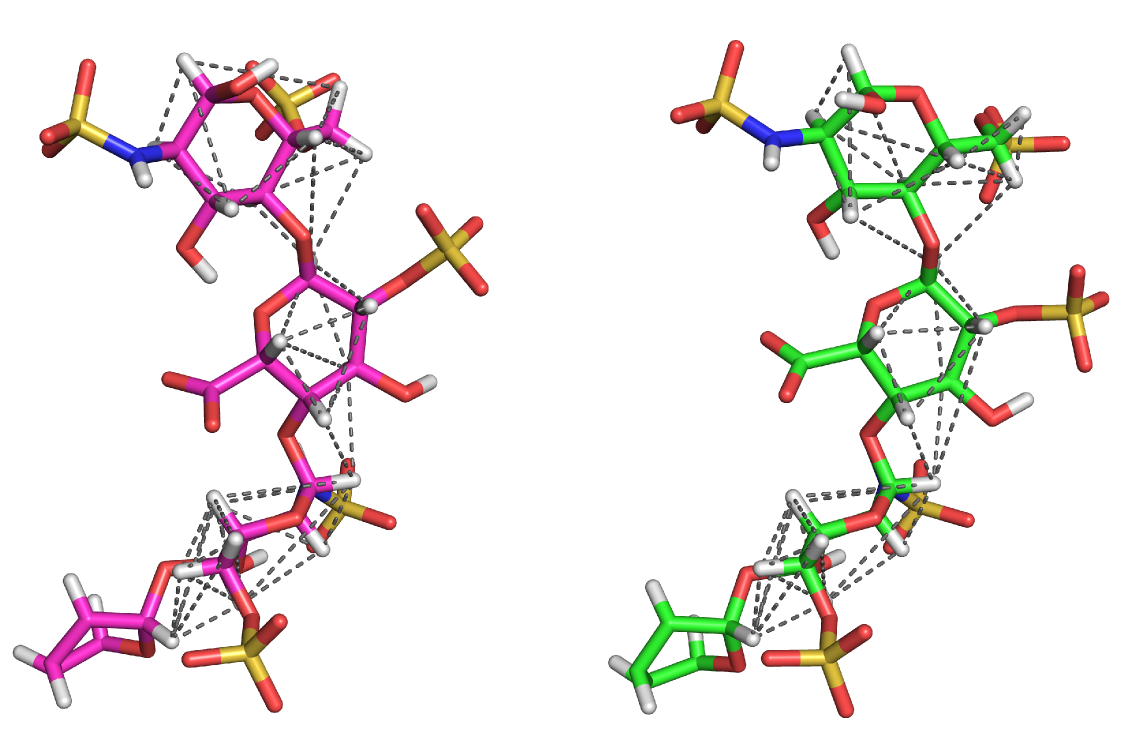
\includegraphics[width=0.7\textwidth]{gfx/nmr/two_cases_dashed_lines_distances.png}
\caption[]{
Heparin tetrasaccharide-internal H-H distance restraints applied during
simulated annealing MD simulations. Each dashed line corresponds to one NMR
distance restraint. In the unbound case (left, carbon in magenta), 42
restraints were applied. In the bound case (right, carbon in green), 41
restraints were used. Functional groups of ring A are not shown for clarity.
Atoms are color-coded with red, blue, yellow, gray corresponding to oxygen,
nitrogen, sulfur, and hydrogen, respectively.
}
\label{fig:nmr:hp_dashed_lines_distances}
\end{figure}

\begin{figure}
\centering
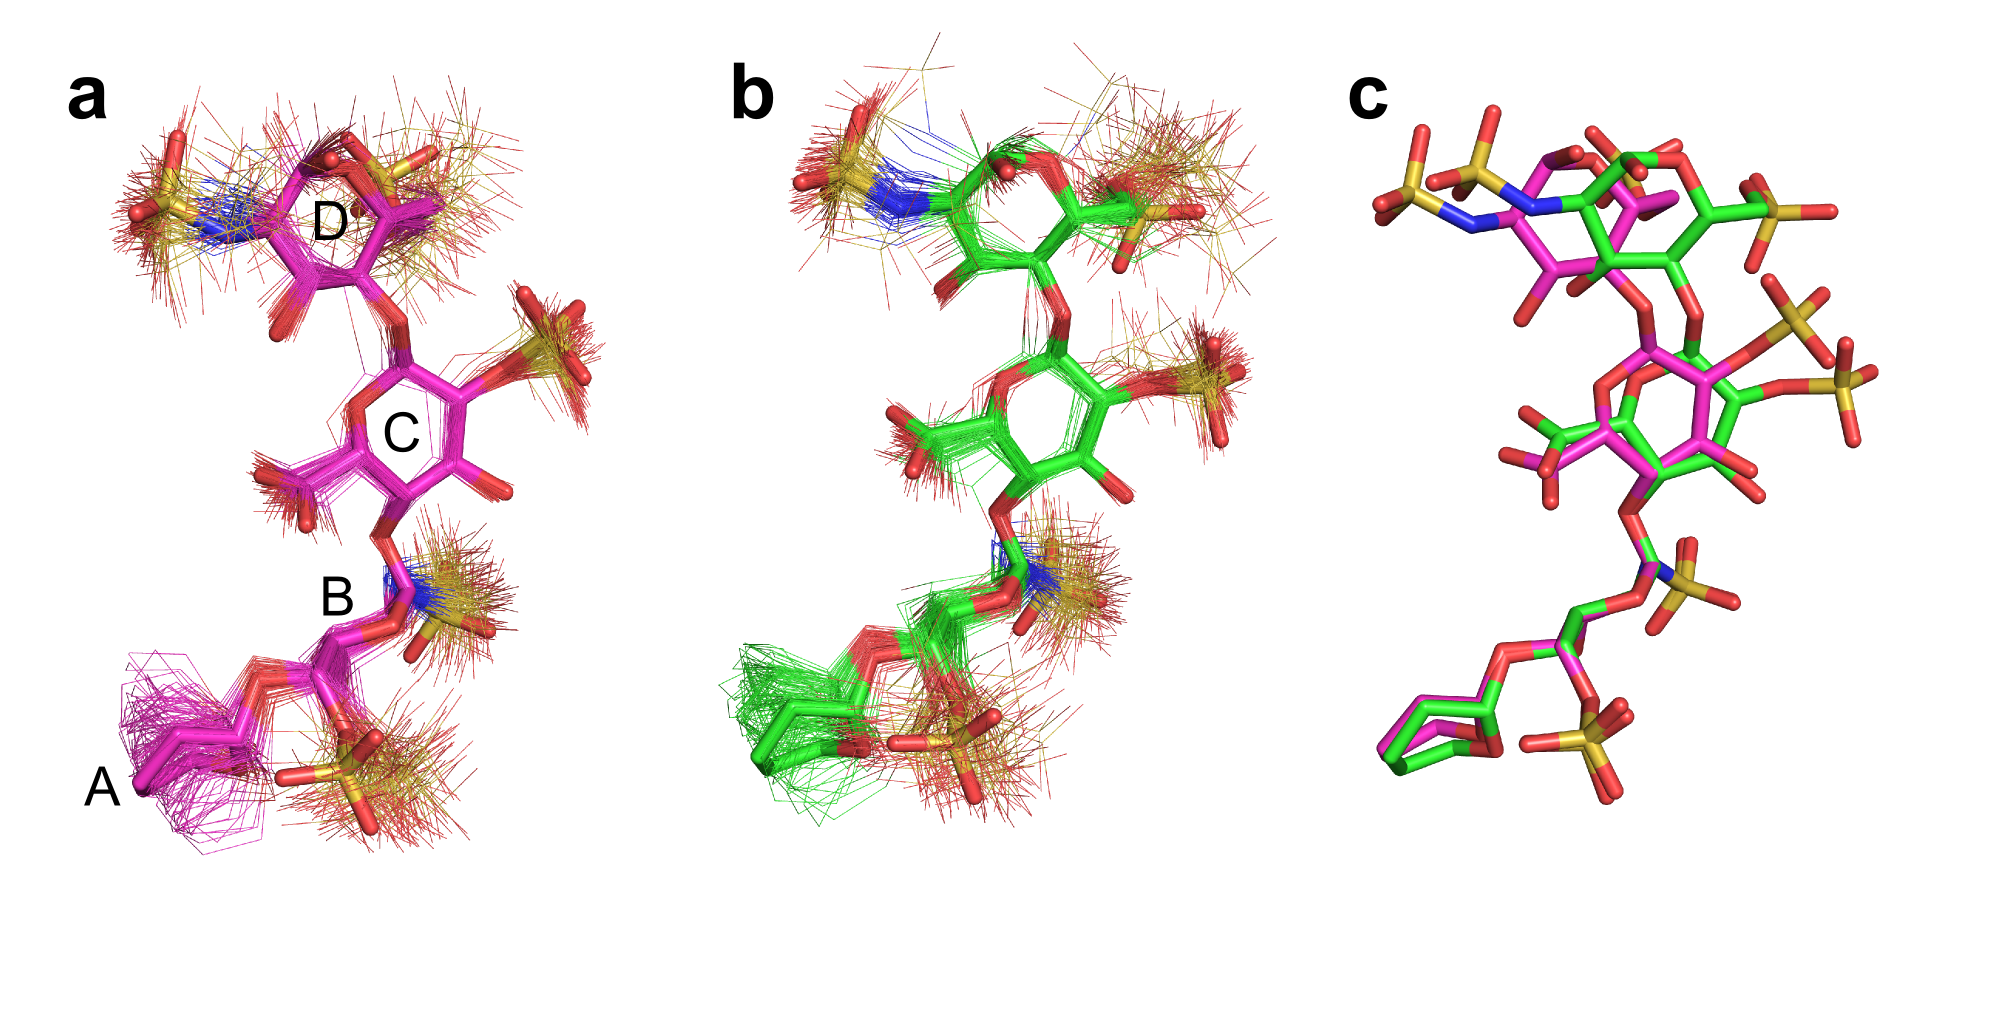
\includegraphics[width=\textwidth]{gfx/nmr/Figure_07_bound_vs_free_three_panels_05.png}
\caption[]{
Heparin structure models obtained from NOE data and simulated annealing
simulations. (a) structure model ensemble for the unbound case (ring identifiers
in capital letters). (b) structure model ensemble for the bound case. (c) the
representative structure for both, the unbound (carbons in magenta) and bound
(carbons in green) ensembles, aligned on ring B. The ensemble representatives
are shown in thick sticks. Functional groups of ring A and hydrogens are not
shown for clarity. Atoms are colored by type (oxygen: red, nitrogen: blue,
sulfur: yellow).
}
\label{fig:nmr:hp_ensembles_representatives}
\end{figure}

Structural models of HP dp4 were created based on NOE data by performing
simulated annealing MD simulations including hydrogen pair distance restraints,
for the unbound HP dp4 and for HP dp4 in the presence of IL-10. In the unbound
case, 42 H-H distance restraints were applied during the simulations (visualized
in \cref{fig:nmr:hp_dashed_lines_distances}). A total of 20 showed a deviation
from the tolerance interval of less than \SI{0.2}{\angstrom}. The ensemble had a
structural diversity of \SI{0.37}{\angstrom}
(\cref{fig:nmr:hp_ensembles_representatives}a). In the bound state, we
restrained the distance of 41 hydrogen pairs, as visualized in
\cref{fig:nmr:hp_dashed_lines_distances}. A total of eight showed a deviation
from the tolerance interval of less than \SI{0.1}{\angstrom}. The resulting
ensemble had a structural diversity of \SI{0.43}{\angstrom}
(\cref{fig:nmr:hp_ensembles_representatives}b). During the structure calculation
we did not apply experimental constraints involving hydrogens of ring A other
than H1 due to inaccurate parameterization of the GLYCAM force field for the
4,5-unsaturated acid ring. Since the ${}^{4,5}\Delta$-uronic acid ring
originates from preparation of the tetrasaccharide by lyase digestion it plays
no functional role for the biology of heparin or heparan sulfate and,
consequently, we do not discuss structural details of this ring --- an approach
which has also been taken in \cite{jin_heparin_2009}. Hence, functional groups
of ring A are not shown in \cref{fig:nmr:hp_ensembles_representatives}. We
quantified the difference in the GAG backbone structure for the bound and
unbound case by evaluating the distribution of glycosidic linkage torsional
angles in both ensembles (\cref{fig:nmr:hp_glyco_dihedral_distributions}). A
significant change in the Φ distribution of linkage A→B, a shift in the Ψ
distribution of linkage B→C, and a significant shift in the Φ distribution of
linkage C→D was observed.


\begin{figure}
\begin{adjustwidth}{-2cm}{-2cm}
\centering
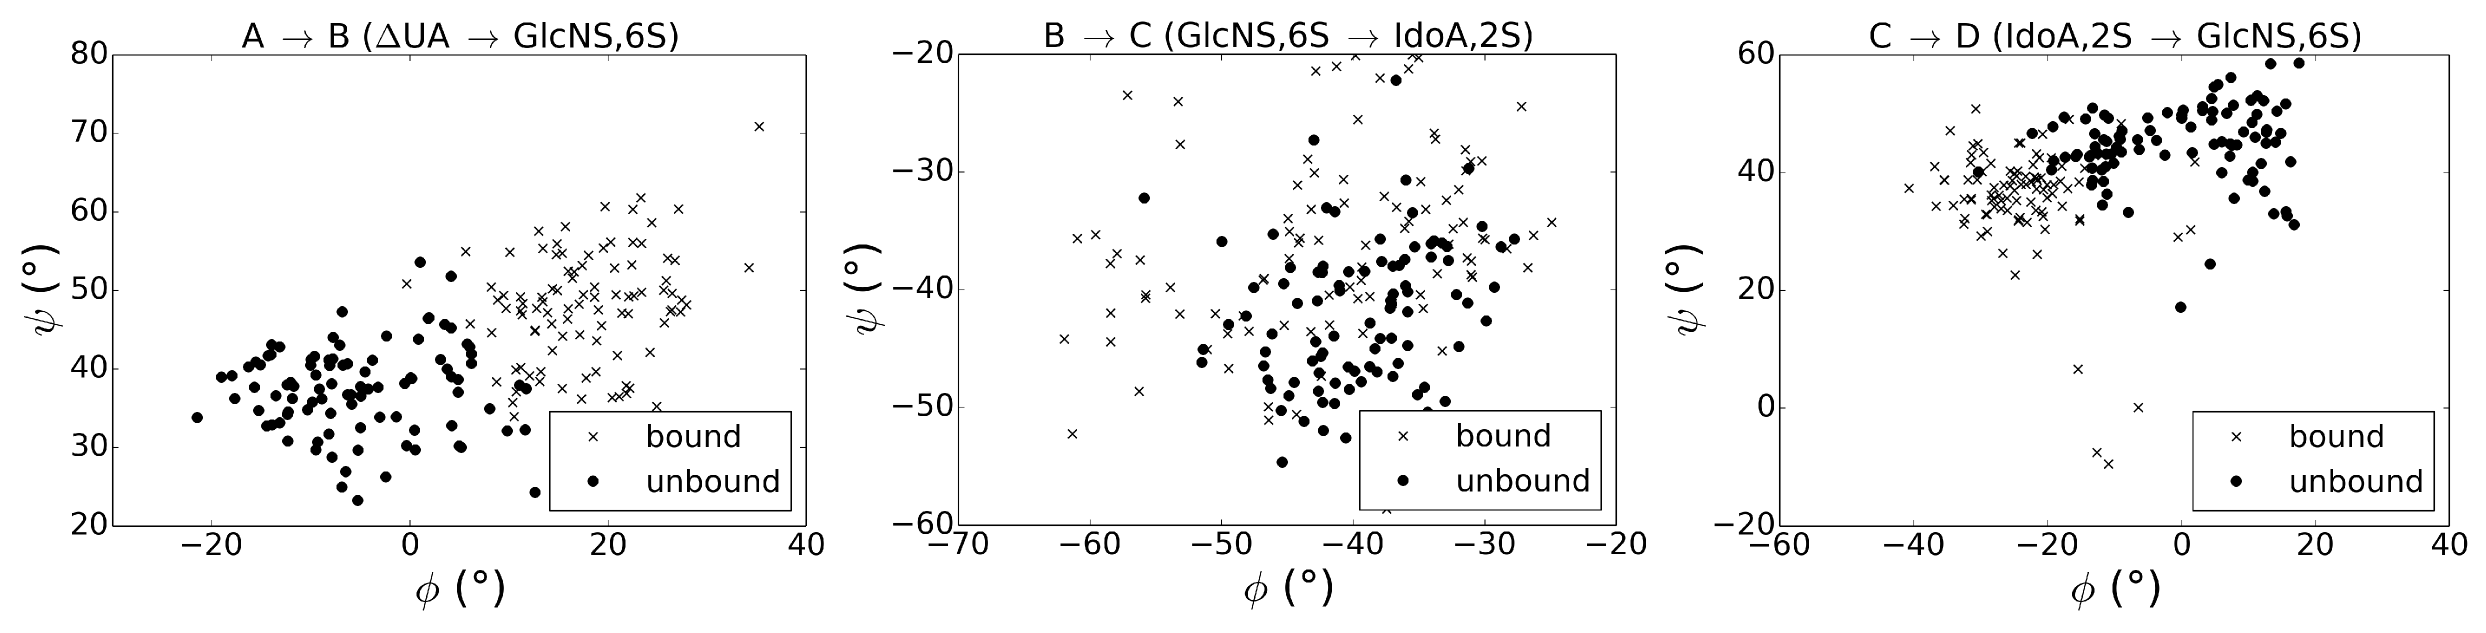
\includegraphics[width=1.3\textwidth]{gfx/nmr/Figure_08_glycolinkage_dihedrals_bound_vs_free_three_3panels_05.png}
\caption[]{
Glycosidic linkage torsional angle distributions of heparin structure model
ensembles obtained from NMR distance restraints and simulated annealing
simulations. Data comparing the bound and unbound state is shown individually
for each linkage in the heparin tetrasaccharide, namely for linkages A
\rightarrow B, B \rightarrow C, and C \rightarrow D.
}
\label{fig:nmr:hp_glyco_dihedral_distributions}
\end{adjustwidth}
\end{figure}

The orientation of four of the six sulfate groups in the tetrasaccharide did not
differ significantly between the bound and unbound state. The orientation of the
6-O-sulfates of the rings B and D, however, was observed to be affected by the
presence of IL-10 (see \cref{fig:nmr:hp_sulfate_orientations}). The 6-O-sulfate
of ring B showed a shift in the rotamer distribution and \SI{10}{\degree}
deviation from the ideal rotation angle of \SI{-60}{\degree}. The 6-O-sulfate of
ring D also populated a small fraction of the \textit{gauche-trans} conformer
(\SI{60}{\degree}) in the presence of IL-10. Further information on the
conformation of 6-O-sulfate side chains was revealed from 3J couplings between
H5 and H6 protons, \hl{as discussed in part...}

\begin{figure}
\centering
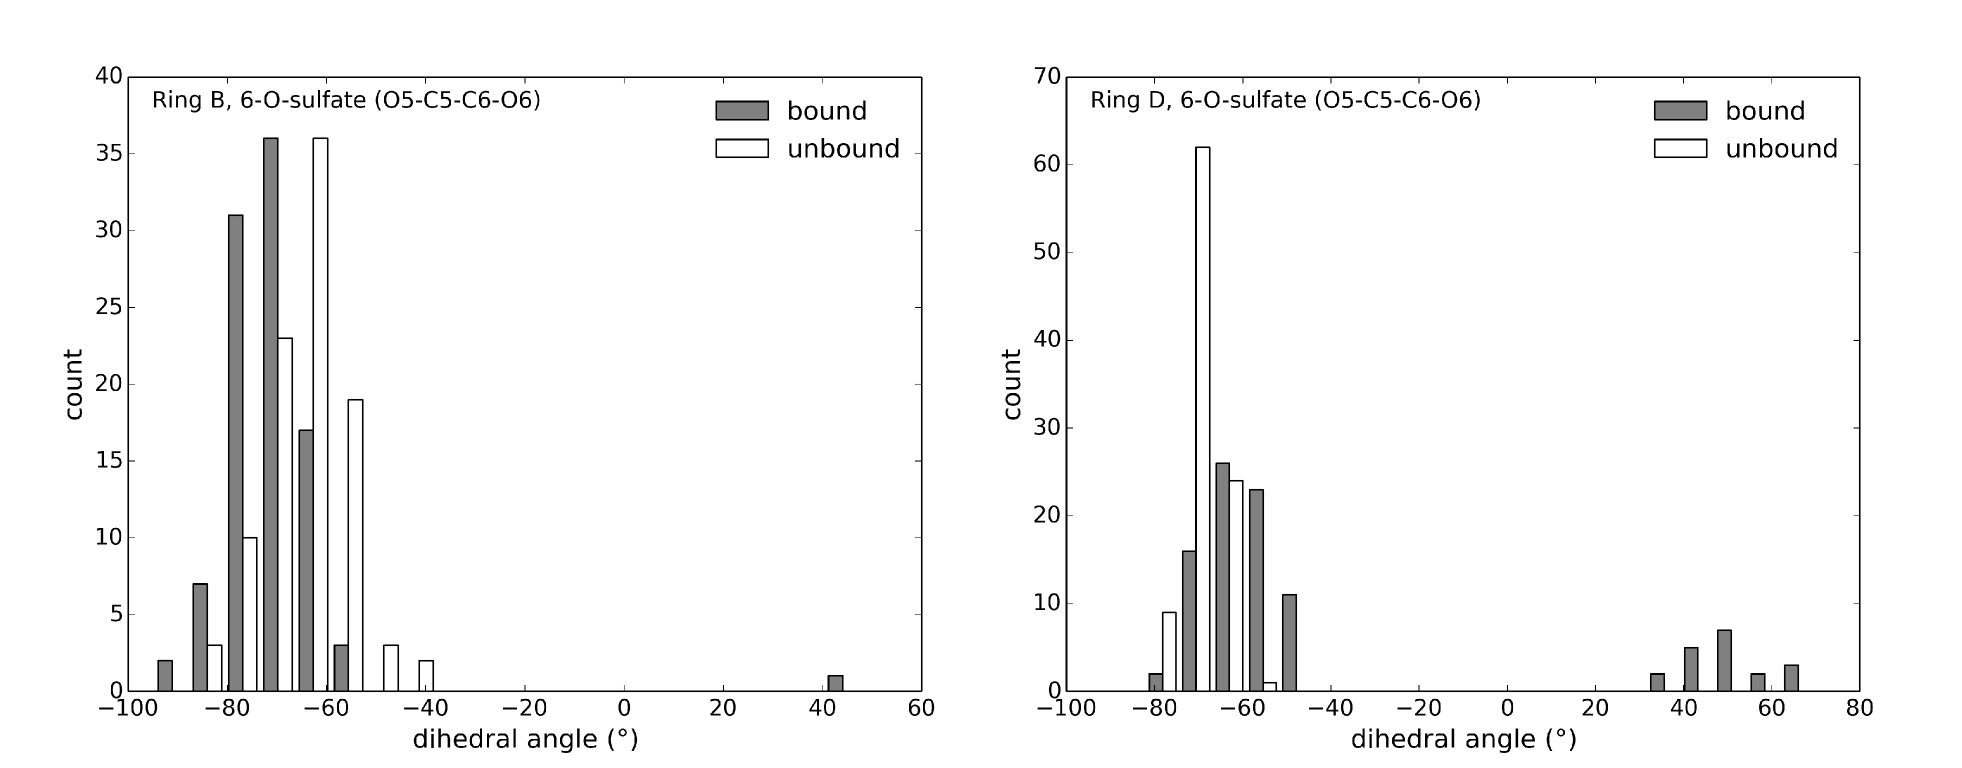
\includegraphics[width=\textwidth]{gfx/nmr/SI_figure_6O_sulfate_dihedrals_B_D_01.png}
\caption[]{
Distribution of 6-O-sulfate orientations in heparin tetrasaccharide structure
models obtained from H-H NMR distance restraints and simulated annealing
simulations, in comparison for the bound and unbound state.
}
\label{fig:nmr:hp_sulfate_orientations}
\end{figure}

The NOE distance data and MD simulations have led to proper heparin structure
models. In both, the bound and unbound case, the ensemble representatives have
their rings in valid conformations, namely ring B in ${}^4$C${}_1$, ring C in
${}^2$S${}_O$, and ring D in ${}^4$C${}_1$ conformation. Also the distribution
of glycosidic linkage torsional angles is in a valid range of values, as
observed in free heparin microsecond MD simulations (data not shown) and in
bound and unbound heparin structures found in the PDB.

The generated structure models let us conclude that the bound heparin structure
is less bent than its free form. The small but significant difference observed
in the backbone structure of the bound and unbound ensembles is reflected by
their glycosidic linkage torsional angle distributions. However, although
glycosidic bond angles between the free and bound state do vary between
\SI{10}{\degree} and \SI{30}{\degree} for linkages A→B and C→D, the overall
tetrasaccharide conformation is maintained and is consistent with the helical
structure of the heparin dodecasaccharide previously observed by NMR and
modelling \cite{foster_mulloy_1993}. Also in the high affinity complex between
bFGF and a heparin tetrasaccharide
\cite{faham_heparin_1996,mikhailov_hp_tetra_1996} the backbone differences
relative to the unbound GAG are rather small and provide no indication about the
interaction strength. Furthermore, according to our heparin structure models,
the orientation of most functional groups of rings B, C, and D is conserved
among the bound and unbound MD ensembles. Notable exceptions are the positions
of the 6-O-sulfate groups of ring B and D. In ring B the 6-O-sulfate is only in
\textit{gauche-gauche}, but there is a slight shift by about \SI{-10}{\degree}
of the rotamer distribution in the bound heparin structure. In ring C an
additional fraction of the \textit {gauche-trans} conformer in the presence of
IL-10 is observed. The observation of the 6-O-sulfate being mostly in \textit
{gauche-gauche} orientation is in contradiction to our \hl{3J} coupling
analysis. The latter estimated the C5-C6 bond in both glucosamine residues to
have \SI{70}{\percent} \textit{gauche- gauche} and \SI{30}{\percent} \textit
{gauche-trans} character as found for other D-glucopyranoses (Nishida et al.
1988). The described contradiction suggests that the sulfate rotamer
distribution as yielded by our MD structure optimization protocol is over-
sensitive to small variations in single distance restraints and that the
interpretation of the 3J coupling data should take precedence.

\hl{Note (TODO):}
\hl{Discuss what this HEPARIN STRUCTURE now brings us for clarifying atomic
detail interaction..}


\section{IL-10-GAG interaction enlightened via NMR}
\hl{Note (TODO):}
\hl{A summary of the remaining major results of Georg's NMR study.}


In \cref{chapter:bspred} we calculated IL-10's Coulomb potential and evaluated
its topology in space, and came up with a putative IL-10-GAG binding region. For
symmetry reasons, this region occurs twice in the IL-10 dimer, separated by a
distance of approximately 30 to 40 Å that is comparable to the length of an
extended GAG decasaccharide. Based on our STD binding data, we hypothesize a
scenario in which an appropriately long GAG molecule could bridge both binding
sites. For a fully sulfated heparin octa- or decasaccharide binding affinity is
nearly 10 or 20-fold higher than for the heparin disaccharide I-S. We interpret
this increase in affinity as effect of positive cooperativity indicated by a
steeper slope of the corresponding binding curves and a Hill coefficient of
around 2. Once the GAG molecule is fixed to one binding site, association with
the second site can happen very fast e.g. due to spatial restriction and thus
affinity is also increased.

\hl{Note (TODO):}
More discussion.
% That discrepancy probably originates from the strong H2-H5 NOE, which is
% dominated by the shorter H2-H5 distance of the 2SO structure (2.4 Å) compared to
% the 1C4 form (4.0 Å) (Mulloy et al. 1993) and thus fixes the monosaccharide in
% skew-boat-conformation during the simulation. In contrast, based on 3J couplings
% we determined the equilibrium between 1C4 and 2So in the IL-10-bound structure
% to be 33 %:67 %. This interesting observation can indicate that either the
% iduronic acid is not interacting with the protein, and thus interconversion of
% the sugar ring can take place, or that two binding modes may exist – one

% with the iduronic acid bound in 1C4 and the other with the iduronate in 2So. For
% some heparinprotein complexes also a conformational selection mechanism has been
% previously suggested. For example, in the crystal structure of annexin V with
% two heparin tetrasaccharide molecules the IdoA,2S ring of molecule 2, which
% interacts with the protein, adopts a 2So conformation whereas the non-
% interacting IdoA,2S ring in the second molecule resides in the 1C4 conformation
% (Capila et al. 2001). Furthermore, for the heparin pentasaccharide AGA*IA(M)
% (GlcNS,6S-GlcA-GlcNS,3S,6S-IdoA,2S-GlcNS,6S-Me) in complex with the FGF-receptor
% 2 (FGFR2) only the 2So conformer of IdoA was observed with NMR as a result of
% conformational selection (Nieto et al. 2011).

% In conclusion, we show that IL-10 is capable of binding a variety of GAG ligands
% for which we delimited their binding epitopes. This molecular recognition
% imposes only minor changes on the overall GAG structure. We find that the
% interaction strength is highly dependent on GAG sulfation, in particular
% N-sulfation. Our results provide information on the interaction properties of
% GAGs and IL-10 that can be taken into account e.g. for the design of tissue-like
% matrix materials in regenerative medicine.

% \section{Binding site determination via Pseudo Contact Shift measurements}
% \hl{Should this be in the thesis? Maybe ONLY prediction would be better,
% leave this for publication.}

%\lipsum[1-5]


Discussion: usually, ... requires full relaxation matrix calculations (\cite{foster_mulloy_1993,mikhailov_hp_tetra_1996}), which also requires more data
to be obtained from the NMR experiments... nevertheless, the analysis as we performed it usually has enough accuracy for obtaining useful results bla bla
\cite{jones_noe_2011}.

